This section describes speech synthesis, voice conversion and replay spoofing attacks and specific implementations.  In general, a spoofed speech signal $s(t)$ is generated from the speech signal of a target speaker $x(t)$.  Whereas the input to a speech synthesis system is a text string, that to voice conversion and replay attacks originates from a third speech signal of a source speaker (spoofer) $y(t)$.  



\subsection{Speech synthesis}
\label{ssec:spsyn}

There is a large variety of speech synthesis algorithms, such as formant, diphone, unit-selection and statistical parametric based approaches, in addition to more recent deep-neural network architectures.  Whatever the approach, the aim is to generate intelligible, natural speech for a given text string $c$. In the context of spoofing, a synthetic speech signal is generated according to:

\begin{equation}
s(t) = g_{x(t)}(c),
\label{eq:tts}
\end{equation}

\noindent where $g_{x(t)}$ denotes a text-to-speech mapping generated by a synthesis system with speech units or acoustic models extracted or learned from the speech signal of a target speaker $x(t)$.  While unit-selection approaches generally require large amounts of speaker-specific data to learn the mapping function $g_{x(t)}$, statistical parametric approaches can synthesize convincing speech signals with the adaptation of well-trained models using relatively small quantities of speaker-specific data.  

Our approach to statistical parametric speech synthesis uses hidden Markov models following the approach described in~\cite{Yamagishi2009}.  The specific implementation uses the HMM-based Speech Synthesis System (HTS)\footnote{http://hts.sp.nitech.ac.jp/} where speech signals are parametrised by STRAIGHT (Speech Transformation and Representation using Adaptive Interpolation of weiGHTed spectrum) features, Mel-cepstrum coefficients and the logarithm of the fundamental frequency (log $F_{0}$) with their delta and acceleration coefficients. Acoustic spectral characteristics and duration probabilities are modelled using multispace distribution hidden semi-Markov models (MSD-HSMM)~\cite{Russell1985}.  Speaker dependent  excitation, spectral and duration models are adapted from corresponding independent models according to a speaker adaptation strategy referred to as constrained structural maximum a posteriori linear regression (CSMAPLR)~\cite{Yamagishi2009a}.  Finally, time domain signals are synthesised using a vocoder based on Mel-logarithmic spectrum approximation (MLSA) filters.  They correspond to STRAIGHT Mel-cepstral coefficients and are driven by a mixed excitation signal and waveforms reconstructed using the pitch synchronous overlap add (PSOLA) method.



\begin{table*}
\renewcommand{\arraystretch}{1.3}
%\ninept
\begin{center}
    \begin{tabular}{ l | c c c c }
    \hline
     	 Attack & Na\"{i}ve impostor &  Replay & Voice conversion & Speech synthesis\\ 
    \hline
Input         & impostor speech  & target speech & impostor speech & text\\
Effort        & zero & low & medium-high & high\\
Effectiveness & low &  \textbf{(?)} & medium-high & high\\
 \hline
\hline
    \end{tabular}
    \caption{Comparison of four different attacks in terms of speech used,  required effort and effectiveness.}
		\label{tab::attacks}
   \end{center}
\end{table*}



\subsection{Voice conversion}
\label{ssec:vconv}

%{\bfseries An equation for $s(t)$ is missing - suggest simply applying IFFT to equation~\ref{eq:conversioneq} with simple explanation regarding OLA}

Voice conversion has been used to explore ASV spoofing since the late 90s~\cite{Pellom1999}.  One successful approaches involves so-called Gaussian-dependent filtering~\cite{Matrouf2005}. Here, the spoofing signal $s(t)$ (or $S(f)$ in the spectral domain) is generated by filtering at the frame level the speech signal of the source or spoofer $y(t)$. In the spectral domain it can be represented as follows:

\begin{equation}
S(f) = \frac{\left|H_{x}(f)\right|}{\left|H_{y}(f)\right|}Y(f)
\label{eq:conversioneq}
\end{equation}

\noindent where $H_{x}(f)$ and $H_{y}(f)$ are the vocal tract transfer functions of the targeted speaker and the spoofer respectively.  $Y(f)$ is the spoofer's speech signal in the spectral domain whereas $S(f)$ denotes the result after voice conversion. A time-domain, converted  signal is recovered as follows:

\begin{equation}
s(t) = IFFT(\frac{\left|H_{x}(f)\right|}{\left|H_{y}(f)\right|})*y(t)
\label{eq:conversioneq_t}
\end{equation}

\noindent where * denotes convolution. As such, $y(t)$ is mapped or converted towards the target in a spectral-envelope sense, and is sufficient to overcome most ASV systems~\ref{Bonastre/Matrouf references}. 

$H_x(f)$ is determined from a set of two Gaussian mixture models (GMMs).  The first, denoted as the automatic speaker recognition (asr) model in the original work, is related to ASV feature space and utilised for the calculation of a posteriori probabilities.  The second, denoted as the filtering (fil) model, is a tied model of linear predictive cepstral coding (LPCC) coefficients from which $H_x(f)$ is derived.  LPCC filter parameters are obtained according to:

\begin{equation}
x_{fil} = \sum\limits_{i=1}^{M}p(g_{asr}^{i}|y_{asr}) \mu_{fil}^{i}
\label{eq:EMit}
\end{equation}

\noindent where $p(g_{asr}^{i}|y_{asr})$ is the a posteriori probability of Gaussian component $g_{asr}^{i}$ given the frame $y_{asr}$ and $\mu_{fil}^{i}$ is the mean of component $g_{fil}^{i}$ which is tied to $g_{asr}^{i}$.  $H_{x}(f)$ is estimated from $x_{fil}$ using an LPCC-to-LPC transformation and a time-domain signal is synthesised from converted frames with a standard overlap-add technique. Full details can be found in~\cite{Matrouf2005, Bonastre2006, Bonastre2007}.


\subsection{Replay}
\label{ssec:replay}

Replay attacks are an example of low-effort spoofing; they require simply the replaying of a previously captured speech signal.  
In the absence of suitable countermeasures and considering the widespread availability of consumer devices with high-quality sound systems, replay attacks can typically be realised with ease.  Furthermore, used either directly, or through the cutting and pasting of short speech intervals, replayed speech has potential to overcome both text-dependent and text-independent ASV systems.  Even though the processes of recording and replaying introduce additive acoustic and convolutive channel and transducer noise, these effects can be attenuated by noise and other intersession (channel) variability compensation techniques common to most modern recognition systems.  These factors point towards the tangible threat posed by replay attacks.

Ignoring ambient noise in the acoustic environment (which is in any case not specific to the replay spoofing scenario), replayed speech can be represented as:


\begin{equation}
s(t) = x(t)*h(t),
\label{eq:replay}
\end{equation}


\noindent where * denotes convolution.  The composite replay effects denoted by $h(t)$ include the impulse responses of replay hardware and the replay environment.  It is composed by:


\begin{figure}
	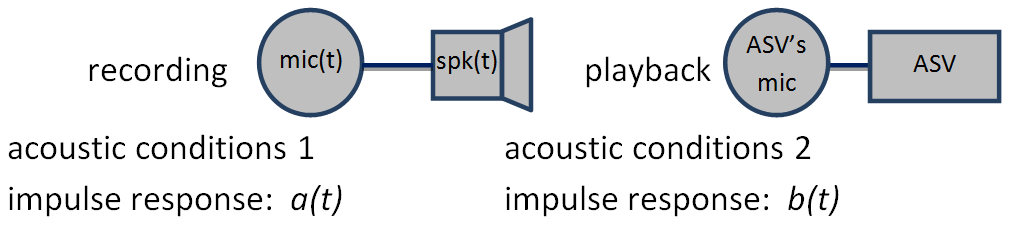
\includegraphics[width=1\linewidth]{Figs/replay.png}
	\caption{A schematic diagram of the assumed replay attack configuration. %{\bfseries <<< Increase font sizes in the figure >>>}%
}
	\label{fig::Replay}
\end{figure}

\begin{equation}
h(t) = mic(t) * a(t) * spk(t) * b(t)
\label{eq::playback}
\end{equation}


\noindent where $mic(t)$ and $spk(t)$ are impulse responses of the microphone and the speaker, respectively, and where $a(t)$ and $b(t)$ are the respective impulse responses of the recording and replay environments.  This scenario is illustrated in Fig.~\ref{fig::Replay}.  Replay attacks may thus be emulated through the convolution of a source signal $s(t)$ with typical impulse responses representing the different replay components.



\subsection{Qualitative comparison}
\label{sec::algorithms::comparison}

Replay, voice conversion and speech synthesis spoofing are forms of \emph{concerted-effort} impostor attacks, as opposed to the na\"{i}ve or \emph{zero-effort} impostor attacks normally used to assess ASV system performance.  A qualitative comparison of all four is illustrated in Table~\ref{tab::attacks}, ordered by the level of effort or expertise needed to implement each attack successfully~\cite{Wu2014a}. 

Compared to na\"{i}ve impostor attacks, replay attacks require slightly increased effort; they require recording and replaying. Voice conversion and speech synthesis attacks require specialised, often complex algorithms, in addition to any recording hardware to collect, analyse and parametrise the target and any other auxiliary speech data.  They belong to a class of higher-effort spoofing attacks.  While voice conversion is based upon the conversion of one speech signal to another, speech synthesis converts a text string to a speech signal, which requires a comparatively higher level of effort or expertise.

One may reasonably suppose that the effectiveness of each attack is correlated with the level of effort involved in their implementation; the higher the effort, the more effective the algorithm and hence the greater the impact on ASV performance.  Replay attacks are then assumed to pose only a low threat.  However, the work in~\cite{Alegre2014} suggests the contrary, showing that replay attacks pose a significant threat, being effective in overcoming an ASV system while being the most easily implemented spoofing attack.  It is the objective of this paper to investigate these contradictory findings and to compare objectively and quantitatively the comparative threat of replay spoofing to those of speech synthesis and voice conversion.
